\section{Garbage collection strategies}

Although the idea of--and the challenges associated with--garbage collection in the context of Irmin differ slightly from what is usually found in litterature, my general approach during this internship was to start by looking there for ideas and algorithms, and then try to adapt them to our problem where relevant. Note that this approach was not always successful, notably because some usual assumptions about garbage collection might not apply to objects stored on Irmin backends which are orders of magnitude slower than RAM--e.g.~\texttt{irmin-fs} or \texttt{irmin-pack}. What follows is a quick summary of the terminology and the classical algorithms from garbage collection literature; and an initial attempt at transposing them to Irmin.

\subsection{Terminology and classical algorithms}

Most of the terminology found in literature~\cite{handbook} can be transposed to Irmin in a straightforward way.

\begin{itemize}
  \item\emph{Objects}.
        An object is either a commit, a node or a blob. Each object is addressed by a hash which is derived deterministically from the content of the object. Objects and their references to each other form a Merkle directed acyclic graph called the \emph{object graph} \(G\).

  \item\emph{Content-addressable heap}.
        The heap is the area in which objects are stored. The precise nature of this area depends on the Irmin backend in use, and how it implements the \texttt{CONTENT\_ADDRESSABLE\_STORE} interface. For instance, objects might be stored in a hashtable in memory; in files on a POSIX filesystem; or in a contiguous array of bytes on a block device.

  \item\emph{Mutator and collector.}
        Following Dijkstra \emph{et al}~\cite{dijkstra78}, garbage-collected systems are usually thought of as a cooperation between two interdependent parts: the \emph{mutator}, which is responsible for the regular operation of the Irmin database--this includes updating the object graph by storing new objects into the heap; and the \emph{collector}, which is responsible for the discovery of unreachable objects in the object graph and their removal from the heap.

  \item\emph{Mutator roots.}
        The \emph{roots} of the mutator are the objects which are directly accessible to the mutator without having to traverse the graph. Depending on the situation, we might want to consider as roots either a specific set of commits, or all the commits which are pointed to by branches in the reference store.

  \item\emph{Reachability.}
        Without surprise, an object is said to be \emph{reachable} if there exists a path in the object graph between the mutator roots and that object. In order for the collector to be safe--see the previous chapter--it is sufficient to ensure that no object gets reclaimed during a collection cycle if it was reachable at the beginning of the cycle.

  \item\emph{Mutator operations.}
        For the sake of simplicity, we reduce the way the mutator operates on the object graph to three functions: \texttt{Store}, which takes an object, stores it on in the heap, and returns its hash; \texttt{Find}, which takes a hash, and returns the object corresponding to this hash from the heap if it exists; and \texttt{Update}, which takes the name of a reference and a hash, and points that reference to that hash. What follows is a trivial pseudo-code implementation of these functions--with \texttt{backend.heap} and \texttt{backend.refs} the content-addressable heap and the reference store of the current backend.

        \begin{verbatim}
Store(o):
    return backend.heap.Set(o)
Find(h):
    return backend.heap.Find(o)
Update(ref, h):
    return backend.refs.Set(ref, h)
\end{verbatim}

  \item\emph{Atomic operations.}
        Since the mutator and collector might operate on the object graph concurrently, some level of synchronization is usually required to avoid race conditions. For the sake of simplicity, the precise mechanism--e.g.~mutexes--will not be specified when writing pseudo-code algorithms. Instead, the keyword \texttt{atomic} will be used to indicate that a series of operations must appear to execute atomically with respect to all others.

\end{itemize}

Broadly speaking, there are two families of garbage collection schemes: those based on \emph{reference counting} and those based on \emph{tracing}.

\subsubsection{Reference counting}

\emph{Reference counting} schemes are based on the fact that an object is reachable if and only if it is a root or if it has at least one predecessor in the graph, so they associate a number called the \emph{reference count} to each object in the heap, and update this count whenever the object gains or looses a predecessor. Eventually, if the count of an object reaches zero, it gets reclaimed--either right away or later on.

\cref{alg:ref-count} is a pseudo-code implementation of reference counting. It extends the behavior of the \texttt{Set} and \texttt{Update} operations defined earlier to keep track of the count for each object and reclaim objects which become unreachable.

\begin{figure}[!ht]
  \caption{Simple reference counting algorithm.}
  \label{alg:ref-count}

  \vspace{-.5em}
  \centering
  \begin{lstlisting}
counts = {}

# Increments the reference count of an object.
increment(o):
    if o $\neq$ null:
        counts[o] $\leftarrow$ counts[o] + 1

# Decrement the reference count of an object, reclaiming the
# object if the count reaches zero–which might recursively
# trigger the reclaiming of successors of the object.
decrement(h):
    if h $\neq$ null:
        counts[h] $\leftarrow$ counts[h] - 1
        if counts[h] = 0:
            for h' $\in$ successors(h):
                decrement(h')
            free(h)

atomic Store(o):
    h $\leftarrow$ backend.heap.Set(o)
    counts[h] $\leftarrow$ 0

    # Update the counts of the successors.
    for h' $\in$ successors(o):
        increment(h')

    return h

atomic Update(ref, new_h):
    old_h $\leftarrow$ backend.refs.Find(ref)
    decrement(old_h)

    backend.refs.Set(ref, new_h)
    increment(new_h)
\end{lstlisting}
\end{figure}


\newpage
However, there are several downsides to reference counting which become problematic under our design constraints. First, it would require storing an integer alongside every object in the content-addressable heap, which would create a significant storage overhead. This integer would also have to be mutable, which would conflict with the current immutable semantics of the heap. Finally, reference counting might impact the performance of other mutator operations negatively and unpredictably--for instance, deleting a branch might trigger a cascade of count updates and object deletions which would result in an unexpected slowdown. For these reasons, I decided to explore tracing-based garbage collection schemes instead.

\subsubsection{Tracing garbage collection}

Instead of keeping track of which objects are reachable \emph{at any point in time} like reference counting schemes, \emph{tracing} schemes wait until the beginning of a collection cycle to traverse the entire object graph from the mutator roots, and find out which objects are reachable. This is an \emph{indirect} approach to garbage collection, as it does not identify garbage directly but rather concludes that every object which was not reached must be garbage.

The most straightforward--and best-known--tracing scheme in literature is \emph{mark-and-sweep}, which was introduced by John McCarthy in 1960 as an implementation consideration for the LISP programming language~\cite{mccarthy60}. It operates in two phases: first the \emph{marking} phase, where it traverses the object graph from the roots and \emph{marks} all the objects it finds; and then the \emph{sweeping} phase, where it iterates over all the objects stored in the heap, reclaims those without a mark, and clears the remaining marks in anticipation for the next collection cycle.

To reason more easily about the state of objects during the marking phase, garbage collection literature usually uses the \emph{tricolor abstraction}~\cite{dijkstra78}, which gives objects a color depending on their current state. At the start of the marking phase, all objects are \emph{white}; when a reachable object has been found, but its successors have not yet been discovered, it becomes \emph{grey}; and when all the successors of a \emph{grey} object have been discovered, it becomes \emph{black}. Eventually, at the end of the marking phase, no grey objects should remain; black objects should be kept; and white objects should be reclaimed as garbage.

\cref{alg:mark-sweep} is a pseudo-code implementation of mark-and-sweep garbage collection using this abstraction. Notice that the \texttt{Collect} function is marked as \texttt{atomic}, and should therefore not execute concurrently with the mutator. In practice, this is achieved by stopping the mutator entirely during collection cycles--otherwise known in literature as ``stopping the world''.

\begin{figure}[!ht]
  \caption{Simple mark-and-sweep collection (adapted from Algorithm 2.1 of \cite{handbook}).}
  \label{alg:mark-sweep}

  \vspace{-.5em}
  \centering
  \begin{lstlisting}
atomic Collect():
    marked $\leftarrow$ mark()
    sweep(marked)

mark():
    marked $\leftarrow$ $\emptyset$           # Set of all the black objects.
    pending $\leftarrow$ Roots()   # Stack of all the grey objects.

    while pending $\neq$ $\emptyset$:
        o $\leftarrow$ pop(pending)
        if hash(o) $\not\in$ marked:
            marked $\leftarrow$ marked $\cup$ {hash(o)}
            pending $\leftarrow$ pending $\cup$ successors(o)

    return marked

sweep(marked):
    for o $\in$ backend.heap.All():
        if hash(o) $\not\in$ marked:
            backend.heap.Free(o)
\end{lstlisting}
\end{figure}


\bigskip
Assuming that \texttt{marked} uses a set data structure with amortized constant-time \texttt{add} and \texttt{find} operations, the \texttt{mark} function is in \(O(n' + m')\) with \(n'\) the number of objects and \(m'\) the number of edges in the subgraph \(G'\) of reachable objects from \(G\), and the \texttt{sweep} function is in \(O(n) * C_{Free}\) with \(n\) the number of objects in \(G\) and \(C_{Free}\) the time complexity of \texttt{Free}--which might vary depending on the implementation.

Generally, mark-and-sweep collectors implement \texttt{Free} by adding the chunks of memory associated with white objects to a \emph{free-list}; and later traversing that list to find areas to allocate new objects to. Although this is sufficient most of the time, the resulting \emph{fragmentation} can be problematic when allocating large objects, as it might become impossible to find a \emph{contiguous} chunk of memory large enough for the object.

To alleviate this issue, schemes such as \emph{sliding compaction}--see Edward's Two-Finger~\cite{saunders74} collector--or \emph{semispace copying} were later introduced. They also operates in two phases: a \emph{marking} phase which is identical to the one in mark-and-sweep; and then a \emph{compaction} or \emph{copying} phase respectively. Although the specifics vary, this second phase rearranges the heap by either moving the black objects next to each other to force the white objects into a single chunk of unused memory; or by splitting it into two semispaces--only one of which is active at a given time--and copying all only the black objects the inactive semispace at the end of each collection cycle, to finally switch the role of the two semispaces atomically.

\subsection{Modular tracing collection}

The modular nature of Irmin leaves us with an interesting problem: as mentioned earlier, our garbage collection scheme should work regardless of the particular storage backend used to implement the heap, but choosing a particular ``flavor'' of tracing collection to implement requires knowing about the specifics of the backend. For instance, if the backend uses a POSIX filesystem to store objects, a classical mark-and-sweep approach works perfectly--simply replace the call to \texttt{Free} in the pseudocode above with a call to \texttt{Unix.unlink}, and let the operating system deal with fragmentation. However, things become more complicated when the backend is a single pack-file since we would have to deal with fragmentation ourselves, so we might want to use semispace-copying instead.

My approach to solving this problem was to notice that all variants of tracing collection can essentially be reduced to a marking phase followed by a ``reclaiming'' phase which uses the object colors assigned during marking to reclaim the space used by white objects. Thus, by factoring out the marking phase and delegating the ``reclaiming'' phase to the backends, we can avoid code duplication while still tailoring to the specific needs of backends.

Practically, this is achieved by extending the interface of backends--\texttt{CONTENT\_ADDRESSABLE\_STORE} to be precise--with a \texttt{filter} function as follows; how the backend implements \texttt{filter} is up to the developer.

\begin{minted}{ocaml}
val filter : t -> (key -> bool) -> unit Lwt.t
(** [filter t p] informs the content-addressable store that it can remove all
    values whose key [k] was added to the store before the call to [filter]
    and does not satisfy the predicate [p]. *)
\end{minted}

Notice that \texttt{filter} receives a \texttt{key\ -\textgreater{}\ bool} predicate returning whether any given object is to be kept or reclaimed, which is a more general approach than simply passing the set of hashes of all the black objects. This approach unfortunately precludes the implementation of garbage collection schemes whose runtime is proportional to the number of reachable objects instead of the total number of objects--see~\cite{zorn90}; but it is a necessary trade-off to allow the implementation of the \emph{partial collection} schemes described in the later chapter on \emph{Memory-constrained marking}.

Notice also that this interface makes no assumptions on the synchronicity of the \texttt{filter} operation: a \texttt{CONTENT\_ADDRESSABLE\_STORE} which receives a call to \texttt{filter} might choose to free up the space occupied by the unreachable objects right away; or instead to wait until a later time--e.g.~to reclaim many objects in batch. This leaves room for the implementation of subtler backend strategies, some of which are described in the later chapter on \emph{Backend filtering strategies}.

Summing up, we get the pseudo-code from \cref{alg:modular-tracing}.

\begin{figure}[!ht]
  \caption{Modular tracing collection.}
  \label{alg:modular-tracing}

  \centering
  \begin{lstlisting}
atomic Collect():
    marked <- mark()
    backend.heap.Filter(λh. h ∈ marked)

mark():
    # Stack of all the grey objects.
    pending <- Roots()

    # Set of all the black objects.
    marked <- ∅

    while pending $\neq$ ∅:
        o <- pop(pending)
        if hash(o) ∉ marked:
            marked <- marked ∪ {hash(o)}
            pending <- pending ∪ successors(o)

    return marked
\end{lstlisting}
\end{figure}


\subsubsection{Implementation details}

The corresponding OCaml implementation is available in \cref{app:modular-tracing}. Notice the use of the \texttt{t.write\_lock} mutex, which is also added to any mutator operation, to ensure the atomicity of collection cycles. To minimize the pause times and the memory overhead of the collector as much as possible, I used memory profiling tools--see \texttt{Spacetime}~\cite{spacetime} and \texttt{prof\_spacetime}~\cite{prof-spacetime}--as well as time profiling and benchmarking tools--see \texttt{ocamlprof}~\cite{ocamlprof} and \texttt{bechamel}~\cite{bechamel} to identify problematic allocations and function calls.

Regarding memory overhead in particular, I ended up implementing the \texttt{marked} set using a \texttt{(key,\ unit)\ Hashtbl.t} instead of the immutable \texttt{key\ Set.t}--from the OCaml standard library--or a third-party hash-set implementation. Although this seems counter-intuitive since the \texttt{unit} type has the same memory footprint as an unboxed integer~\cite{ocaml-layout}, memory profiling showed no significant difference in the amount of memory allocated between a \texttt{(key,\ unit)\
  Hashtbl.t} and the other options mentioned above; while, on the contrary, the runtime of the mutable hashtable was better than the immutable set.

% TODO: Give figures from the benchmark.

\bigskip
Theoretically speaking, the amount of memory necessary to store \(n\) pairs into a \texttt{(\textquotesingle{}k,\ \textquotesingle{}v)\ Hashtbl.t} with a uniformly distributed hash function can be approximated--using the implementation from~\cite{impl-hashtbl}--by the following formula: \[
  size(\texttt{('k, 'v) Hashtbl.t}) = 3 * size(\texttt{int}) + n * (size(\texttt{'k}) + size(\texttt{'v}) + size(\texttt{ptr}))
\]

And the amount of memory necessary to store \(n\) values into a \texttt{\textquotesingle{}v\ Stack.t} can be approximated--using the implementation from~\cite{impl-stack}--by the following formula: \[
  size(\texttt{'v Stack.t}) = size(\texttt{int}) + n * (size(\texttt{'v}) + size(\texttt{ptr}))
\]

Assuming that we are using a 64-bit system, and given that object hashes are 256-bit digests with an extra 8 bytes--as they are wrapped into a variant which indicates the type of the object, we can use these formulas to compute the approximate usage of \texttt{marked} and \texttt{pending}: \[
  \begin{array}{lll}
    size(\texttt{marked})  & = 3*8 + n * (32 + 8 + 8 + 8) & \simeq 56 n \
    \text{bytes}
    \\
    size(\texttt{pending}) & = 1*8 + n * (32 + 8 + 8)     & \simeq 48 n \
    \text{bytes}
    \\
  \end{array}
\]

\bigskip
In other words, calling \texttt{mark} on a graph with a million reachable objects would require at least \(56 MB\) of memory for \texttt{marked}, plus a maximum temporary overhead of of \(48L\) bytes for \texttt{pending} with \(L\) the maximum length of a path in the graph. For more details on what this implies, see the later chapter on \emph{Memory-constrained marking}.

As for runtime, it was previously mentioned that \texttt{mark} theoretically runs in \(O(n' + m')\)--with \(n'\) the number of objects and \(m'\) the number of edges in the subgraph \(G'\) of reachable objects from \(G\). This is confirmed in practice, as the benchmark from \cref{fig:mark-benchmark} shows that the runtime of \texttt{mark} is linear in the number of objects in the graph. Notice that the coefficient varies depending on the backend currently being used--which makes sense, since fetching the objects on disk is obviously slower than in memory.

\begin{figure}[ht]
  \caption{Runtime of \texttt{mark} depending on the backend and the number of objects in the heap.}
  \label{fig:mark-benchmark}

  \centering
  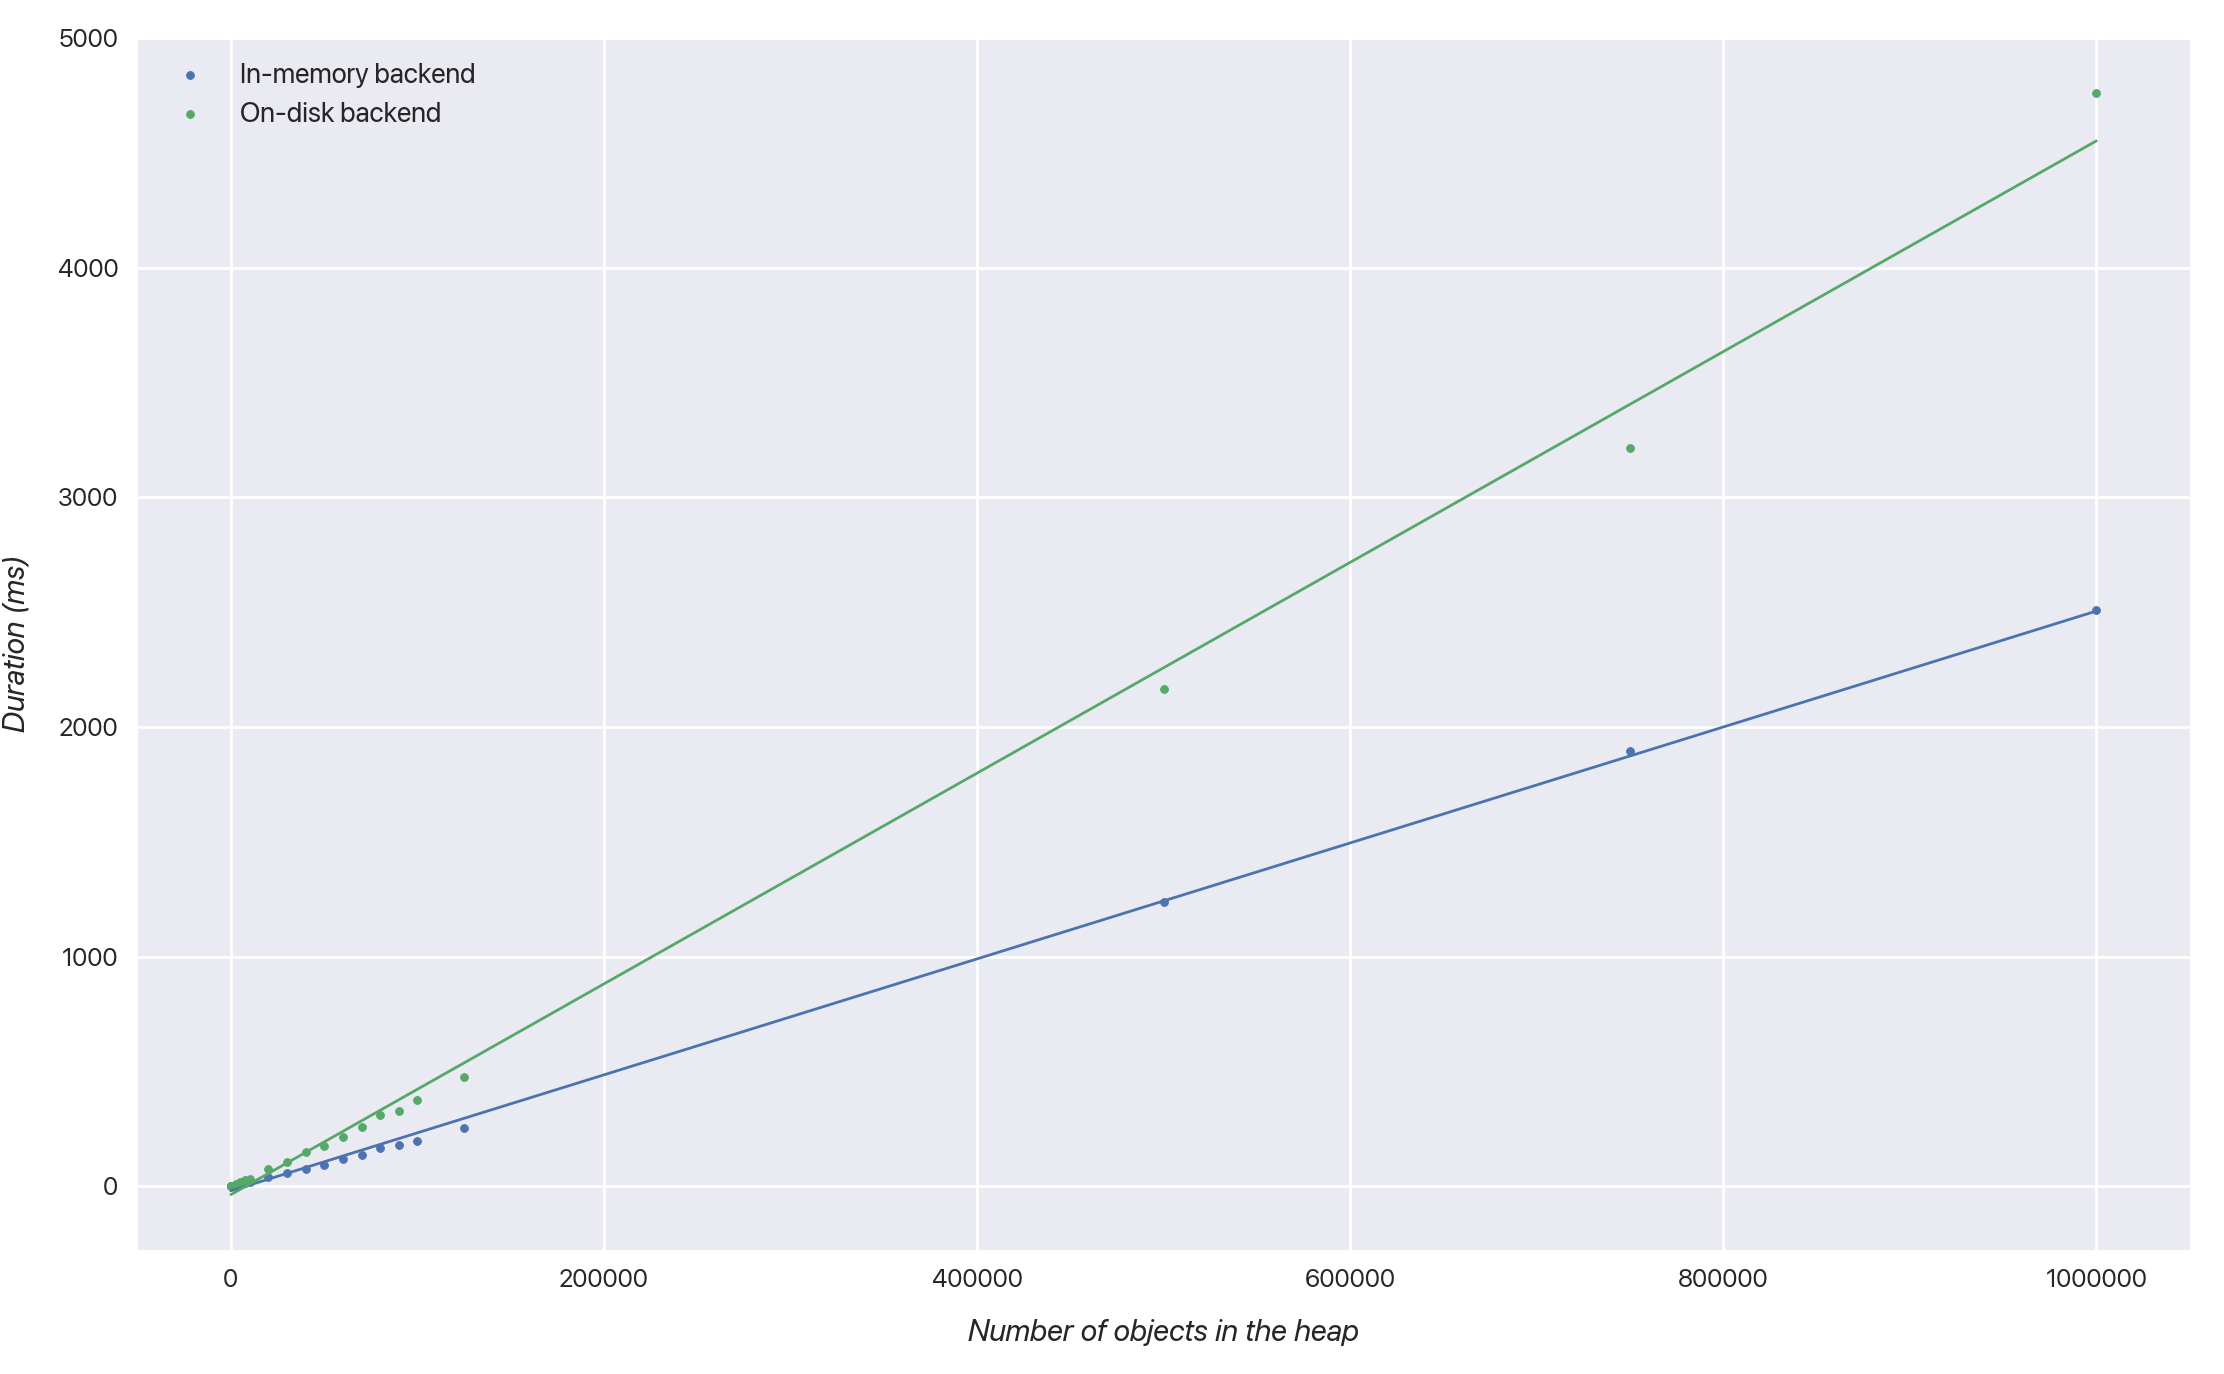
\includegraphics[width=\textwidth]{images/mark_bench.png}
\end{figure}
